% !TeX encoding = UTF-8
% !TeX root = resumo.tex
% !TeX spellcheck = pt_PT

%---------------------------------------------------------------------------------------------------
% Preâmbulo
%---------------------------------------------------------------------------------------------------

\documentclass[9pt,a4paper]{extarticle}

\usepackage[portuguese]{babel}
\usepackage{graphicx}
\usepackage[T1]{fontenc}
\usepackage{times}
\usepackage[utf8]{inputenc}
\usepackage{url}
\usepackage{multicol}
\usepackage{float}
\usepackage[tableposition=top]{caption}
\usepackage{indentfirst}
\usepackage[a4paper,margin=30mm,noheadfoot]{geometry}
\usepackage[noabbrev,nameinlink]{cleveref}

\columnsep 12mm
\pagestyle{empty}
\captionsetup{figurename=Fig.,tablename=Tab.,labelsep=endash,font=bf,skip=.5\baselineskip,justification=centering}

\makeatletter
\renewcommand*{\@seccntformat}[1]{%
  \csname the#1\endcsname.\quad
}
\makeatother

\clubpenalty=300
\widowpenalty=300

\graphicspath{{figures/}}
\setlength{\belowcaptionskip}{-7pt}


%---------------------------------------------------------------------------------------------------
% Cabeçalho
%---------------------------------------------------------------------------------------------------


\begin{document}

\begin{center}
  \huge{\textbf{\textsc{Localiação de robôs em ambientes dinâmicos}}}\\[4mm]
  \Large{\emph{Carlos Miguel Correia da Costa}}\\[2mm]
  \normalsize{Dissertação desenvolvida sob a supervisão do \emph{Doutor Armando Jorge Miranda de Sousa}\\e co-supervisão do \emph{Doutor Germano Manuel Correia dos Santos Veiga}}\\
  \normalsize{no \emph{Centro de Robotica e Sistemas Inteligentes do INESC-TEC}}
\end{center}

\thispagestyle{empty}
\vspace*{-4mm}\noindent\rule{\textwidth}{0.4pt}\vspace*{4mm}



%---------------------------------------------------------------------------------------------------
% Resumo
%---------------------------------------------------------------------------------------------------


\begin{multicols}{2}

\section{Contexto}

A humanidade tem procurado um método confiável de navegação desde que começou a explorar o mundo. Inicialmente a extração de pontos de referência do ambiente eram a única forma de se efetuarem viagens de curta distância. Mais tarde aperfeiçoou-se a navegação astronómica para viagens mais longas e quando a humanidade se aventurou para viagens espaciais, implementou-se um sistema de localização global. Robôs autónomos enfrentam o mesmo problema, dado que para poderem navegar com precisão, precisam de saber a sua localização no ambiente e serem tolerantes a objetos dinâmicos. Ao longo dos anos, vários métodos têm sido propostos para localização de robôs de acordo com o ambiente de navegação e os requisitos de precisão. Alguns foram desenvolvidos para navegação local com elevada precisão enquanto outros fornecem uma posição global aproximada.

Um robô capaz de operar com segurança e precisão em ambientes dinâmicos pode ter inúmeras aplicações, que vão desde tarefas simples de entrega de objetos até operações de montagem avançadas. Além de melhorar a produtividade através da realização de trabalhos repetitivos com precisão e velocidade, os robôs podem também cooperar com humanos para melhorar a eficiência global das tarefas e assim reduzir os custos de produção.


\section{Projeto}

CARLoS\footnote{\url{http://carlosproject.eu/}} é um projeto de investigação europeu que visa o desenvolvimento de um robô autónomo capaz de cooperar com humanos na realização de tarefas repetitivas em ambientes dinâmicos, tais como soldagem de pinos e projeção de informação CAD. Soldadura de pinos é uma tarefa repetitiva que visa fornecer a estrutura de suporte para outros componentes, tais como camadas de isolamento térmico ou sistemas elétricos. Projeção de informação CAD destina-se a ajudar trabalhadores humanos a montar componentes mais rapidamente.


\section{Motivação e objetivos}

Com o aumento da oferta de produtos e serviços devido à constante inovação e globalização dos mercados, as empresas estão a tentar reduzir os custos de produção e a melhorar a produtividade dos seus trabalhadores. Os robôs podem ajudar a alcançar esses objetivos ao permitirem a execução de tarefas repetitivas com alta precisão e velocidade, enquanto os seres humanos se dedicam a tarefas mais complexas e criativas.

Plataformas móveis equipadas com braços robóticos fornecem uma maneira flexível para automatizar uma ampla gama de tarefas. No entanto, para executar as operações pretendidas, os robôs precisam de saber onde estão no ambiente e que caminho devem seguir para chegarem ao local de trabalho definido. Além disso, dado os recursos limitados de energia e de poder computacional, as plataformas móveis robóticas exigem sistemas de controlo eficientes, confiáveis e precisos, para poderem ser capazes de operar em tempo real.


\section{Contribuições}

Durante esta dissertação foi desenvolvido um sistema de localização 3/6 DoF eficiente, modular e extensível \footnote{\url{https://github.com/carlosmccosta/dynamic_robot_localization}} para plataformas robóticas móveis, capaz de funcionar com precisão e confiabilidade em ambientes dinâmicos. É um sistema adaptativo que usa características geométricas para estimar a posição inicial do robô e algoritmos de registo de nuvem de pontos para seguir a sua pose. O subsistema de rastreamento da pose pode ter duas configurações diferentes. Um configurado para o máximo de eficiência e usado para o funcionamento típico da plataforma móvel e outro para situações mais esporádicas que podem exigir algoritmos mais robustos e mais exigentes em termos de poder computacional. Para além de localização, o sistema também suporta a atualização incremental do mapa do ambiente e pode ajustar a sua taxa de operação de acordo com a velocidade estimada do robô. Para operações críticas, é fornecido uma análise detalhada da qualidade do rastreamento da pose e quando é feita uma estimação da pose inicial do robô é fornecida a distribuição das poses aceitáveis, de forma a que um supervisor do sistema de localização detete a existência de lugares com geometria semelhante e planei um caminho que permita desambiguar a pose global do robô.


\section{Plataformas de teste}

O sistema de localização foi testado em dados de sensores laser obtidos a partir de três robôs móveis (mostrados da figura 1 à figura 4) e também a partir de um Kinect. Os testes foram realizados no mesmo computador, a fim de permitir uma comparação direta do tempo de computação. Este computador foi um portátil Clevo P370EM3 (com uma CPU i7 3630QM Intel Core a 2.4GHz, 16 GB de memória RAM DDR3, placa gráfica NVidia GTX680M e um disco Samsung SSD 840 Pro) configurado com Ubuntu 12.04, ROS Hydro, PCL 1,7 e Gazebo 1.9.

Os dados dos sensor foram gravado em rosbags, e estão disponíveis publicamente em \footnote{\url{https://github.com/carlosmccosta/dynamic_robot_localization_tests}} juntamente com todos os resultados e vídeos das experiências, a fim de permitir futuras comparações com outros sistemas de localização.

\vspace{-7pt}
\begin{figure}[H]
	\centering
	\begin{minipage}[b]{0.23\textwidth}
		\centering
		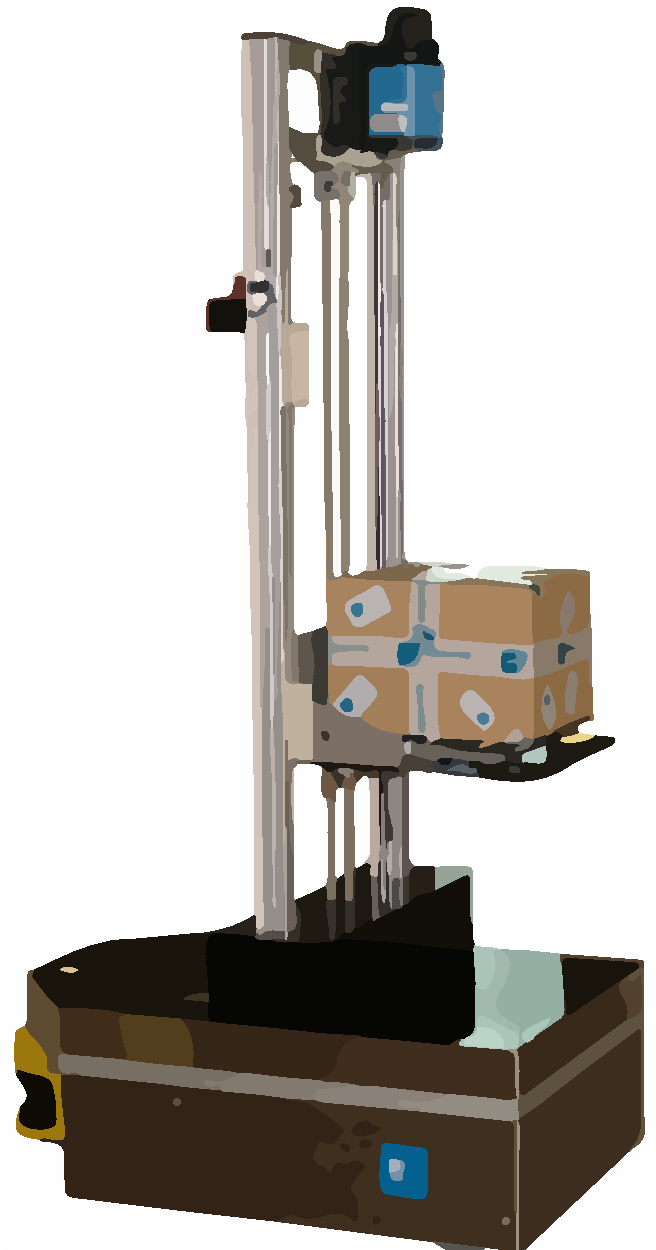
\includegraphics[width=0.4\textwidth]{jarvis}
		\caption{\small Robô Jarvis}
		\label{fig:jarvis}
	\end{minipage}\hfill
	\begin{minipage}[b]{0.23\textwidth}
		\centering
		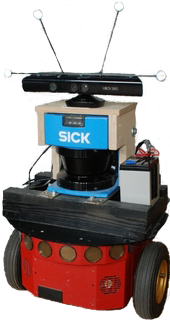
\includegraphics[width=0.3\textwidth]{pioneer-3dx}
		\caption{\small Robô Pioneer \cite{Sturm2012}}
		\label{fig:pioneer}
	\end{minipage}
\end{figure}

\vspace{-9pt}
\begin{figure}[H]
	\centering
	\begin{minipage}[b]{0.2\textwidth}
		\centering
		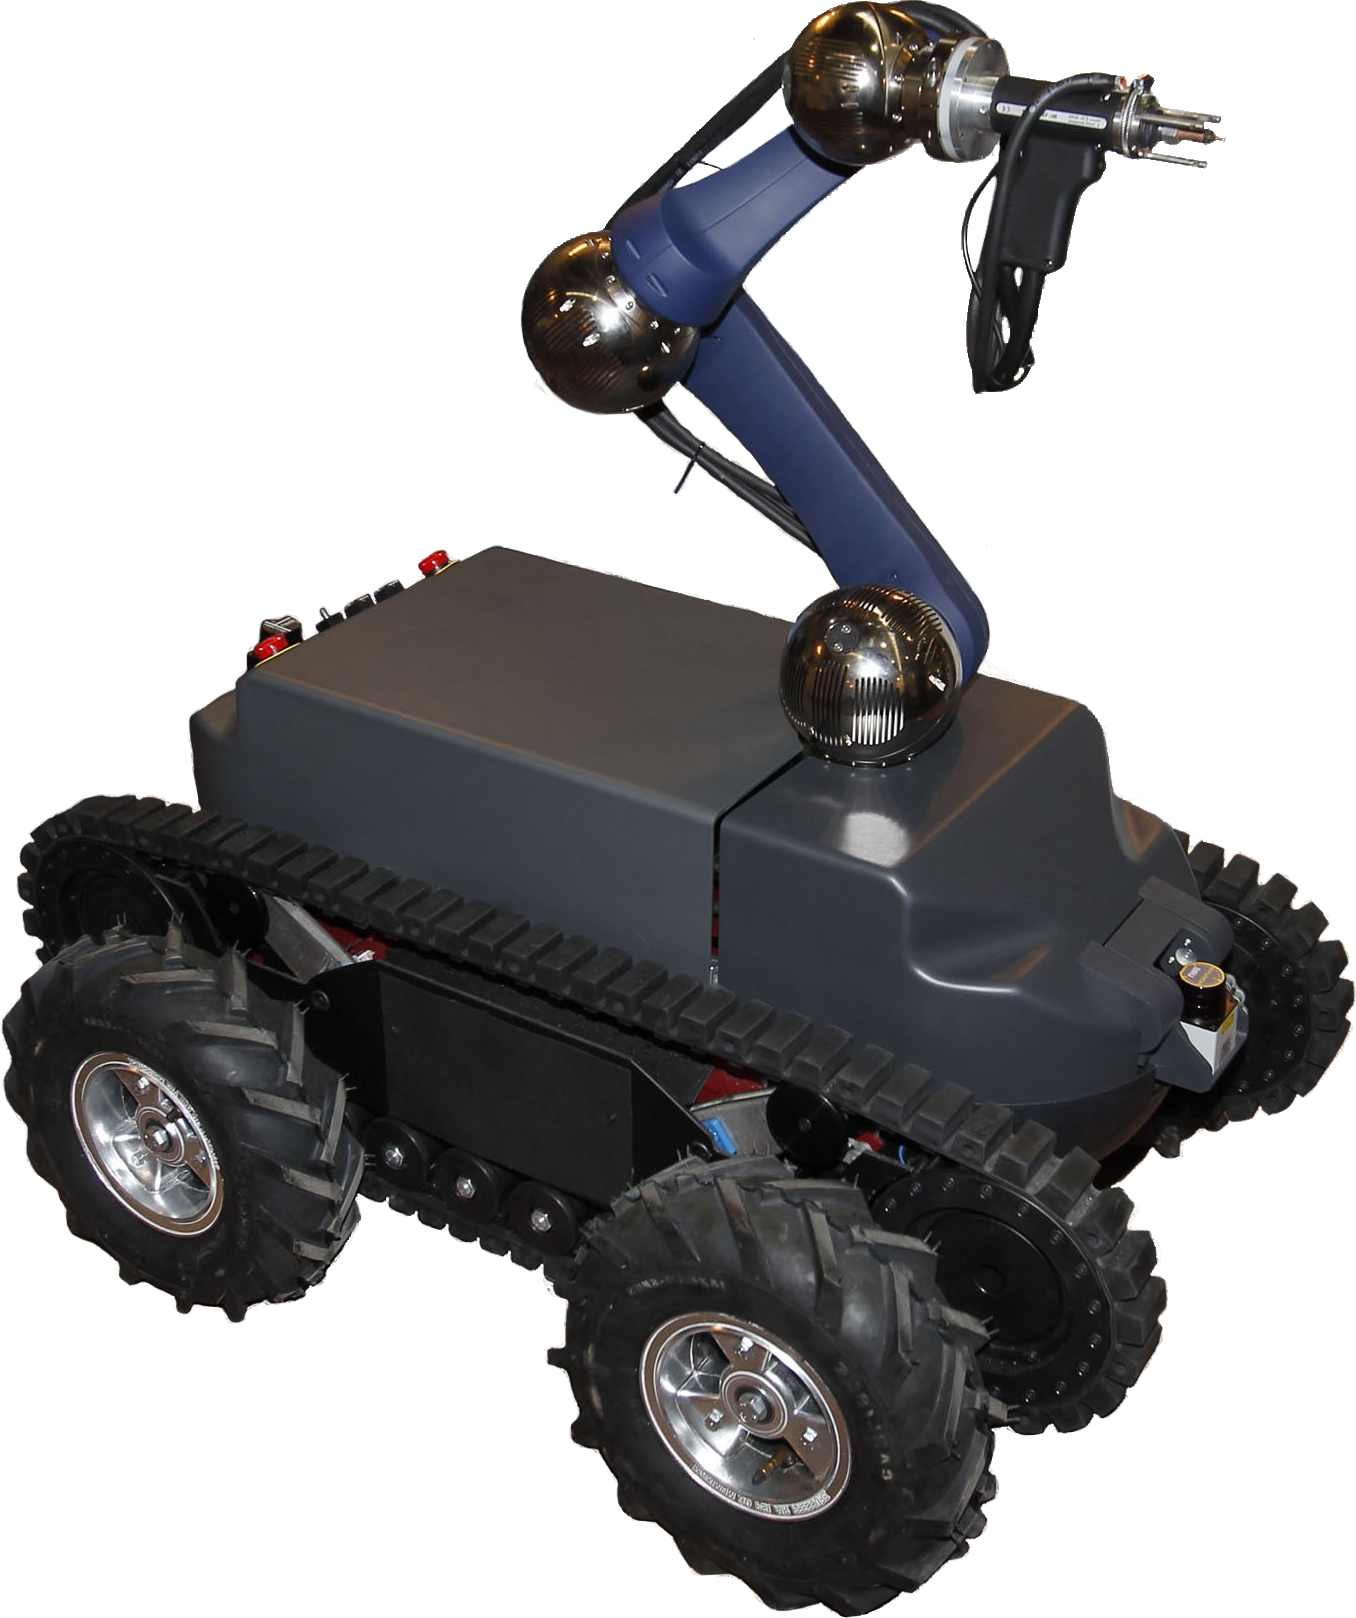
\includegraphics[width=0.6\textwidth]{guardian}
		\caption{\small Robô Guardian}
		\label{fig:guardian}
	\end{minipage}\hfill
	\begin{minipage}[b]{0.25\textwidth}
		\centering
		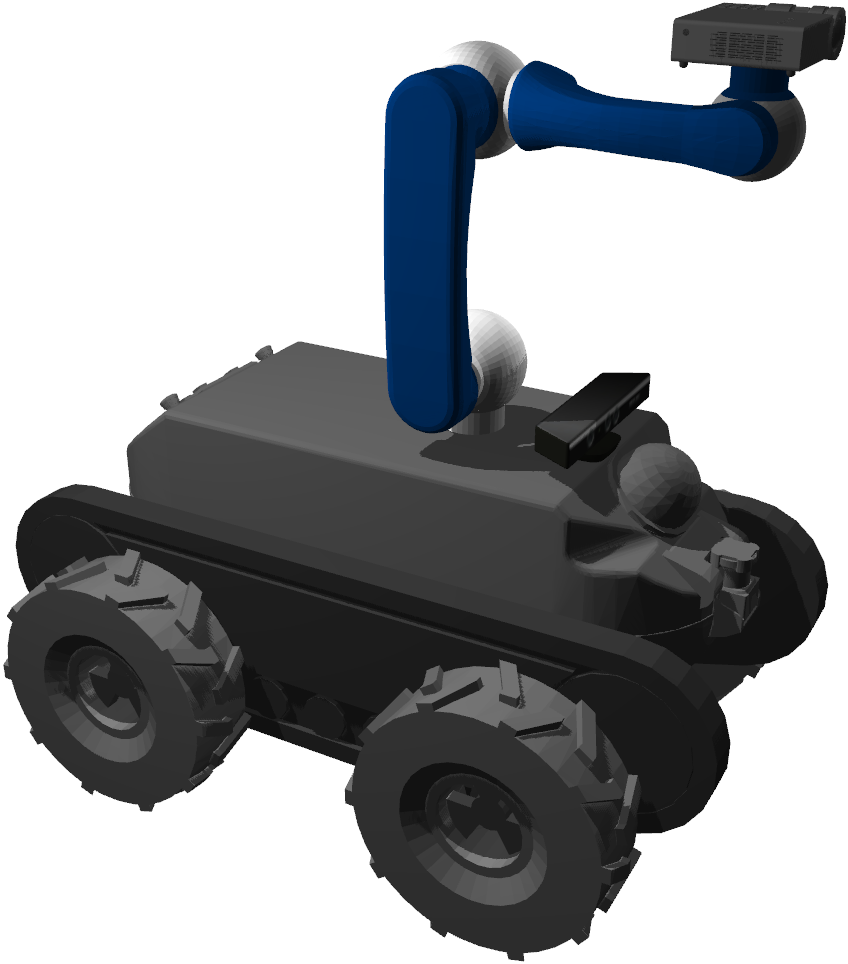
\includegraphics[width=0.45\textwidth]{guardian-gazebo}
		\caption{\small Simulação Guardian}
		\label{fig:guardian-gazebo}
	\end{minipage}
\end{figure}


\section{Ambientes de teste}

O sistema de localização foi testado em diferentes ambientes (mostrados da figura 5 à 8) e usou a plataforma Jarvis numa sala com um campo RoboCup, o Pioneer 3-DX num espaço industrial, a plataforma Guardian num ambiente interior simulado e um Kinect numa arena de voo.


\vspace{-7pt}
\begin{figure}[H]
	\centering
	\begin{minipage}[t]{0.23\textwidth}
		\centering
		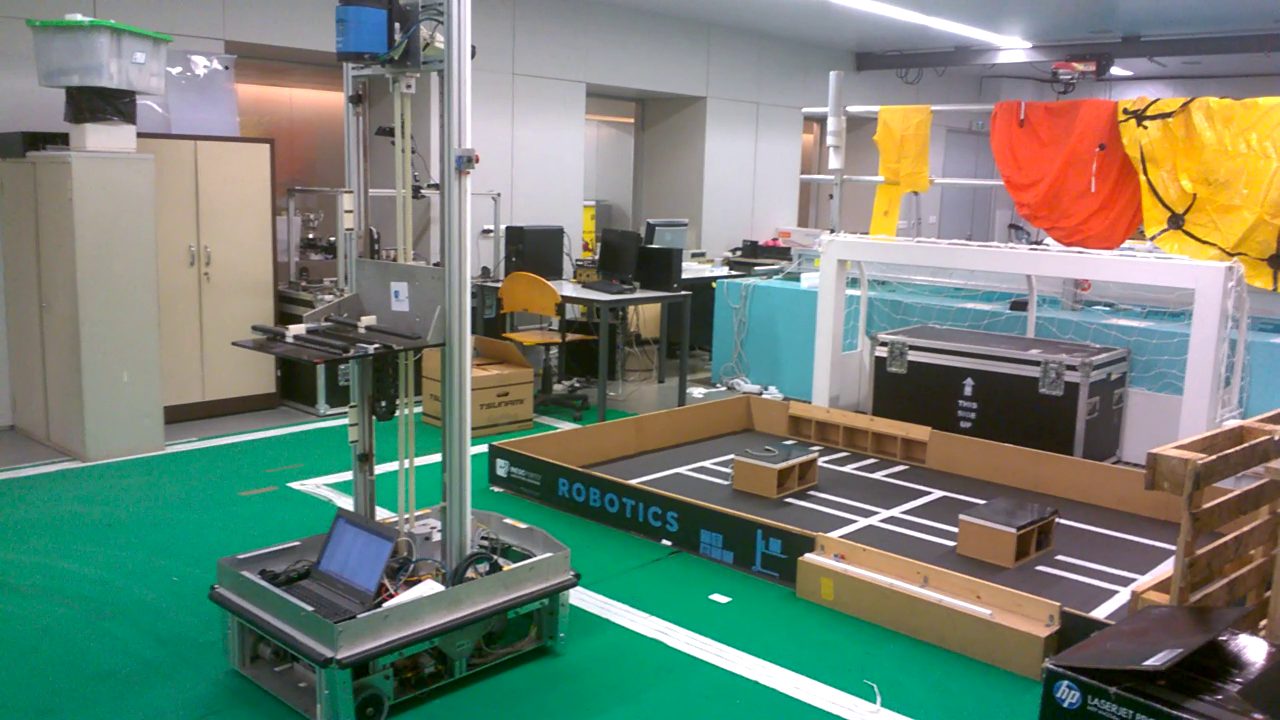
\includegraphics[width=\textwidth]{jarvis-environment-front-right}
		\caption{\small Campo RoboCup}
		\label{fig:jarvis-environment}
	\end{minipage}\hfill
	\begin{minipage}[t]{0.217\textwidth}
		\centering
		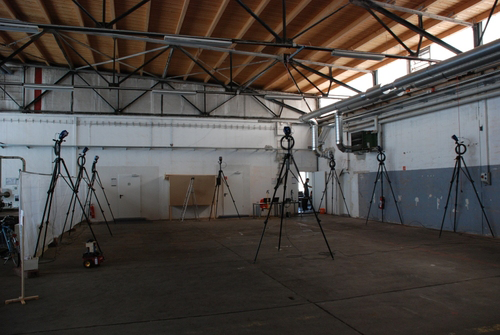
\includegraphics[width=0.9\textwidth]{industrial-hall}
		\caption{\small Ambiente industrial \cite{Sturm2012}}
		\label{fig:pioneer-environment}
	\end{minipage}
\end{figure}


\vspace{-9pt}
\begin{figure}[H]
	\centering
	\begin{minipage}[b]{0.23\textwidth}
		\centering
		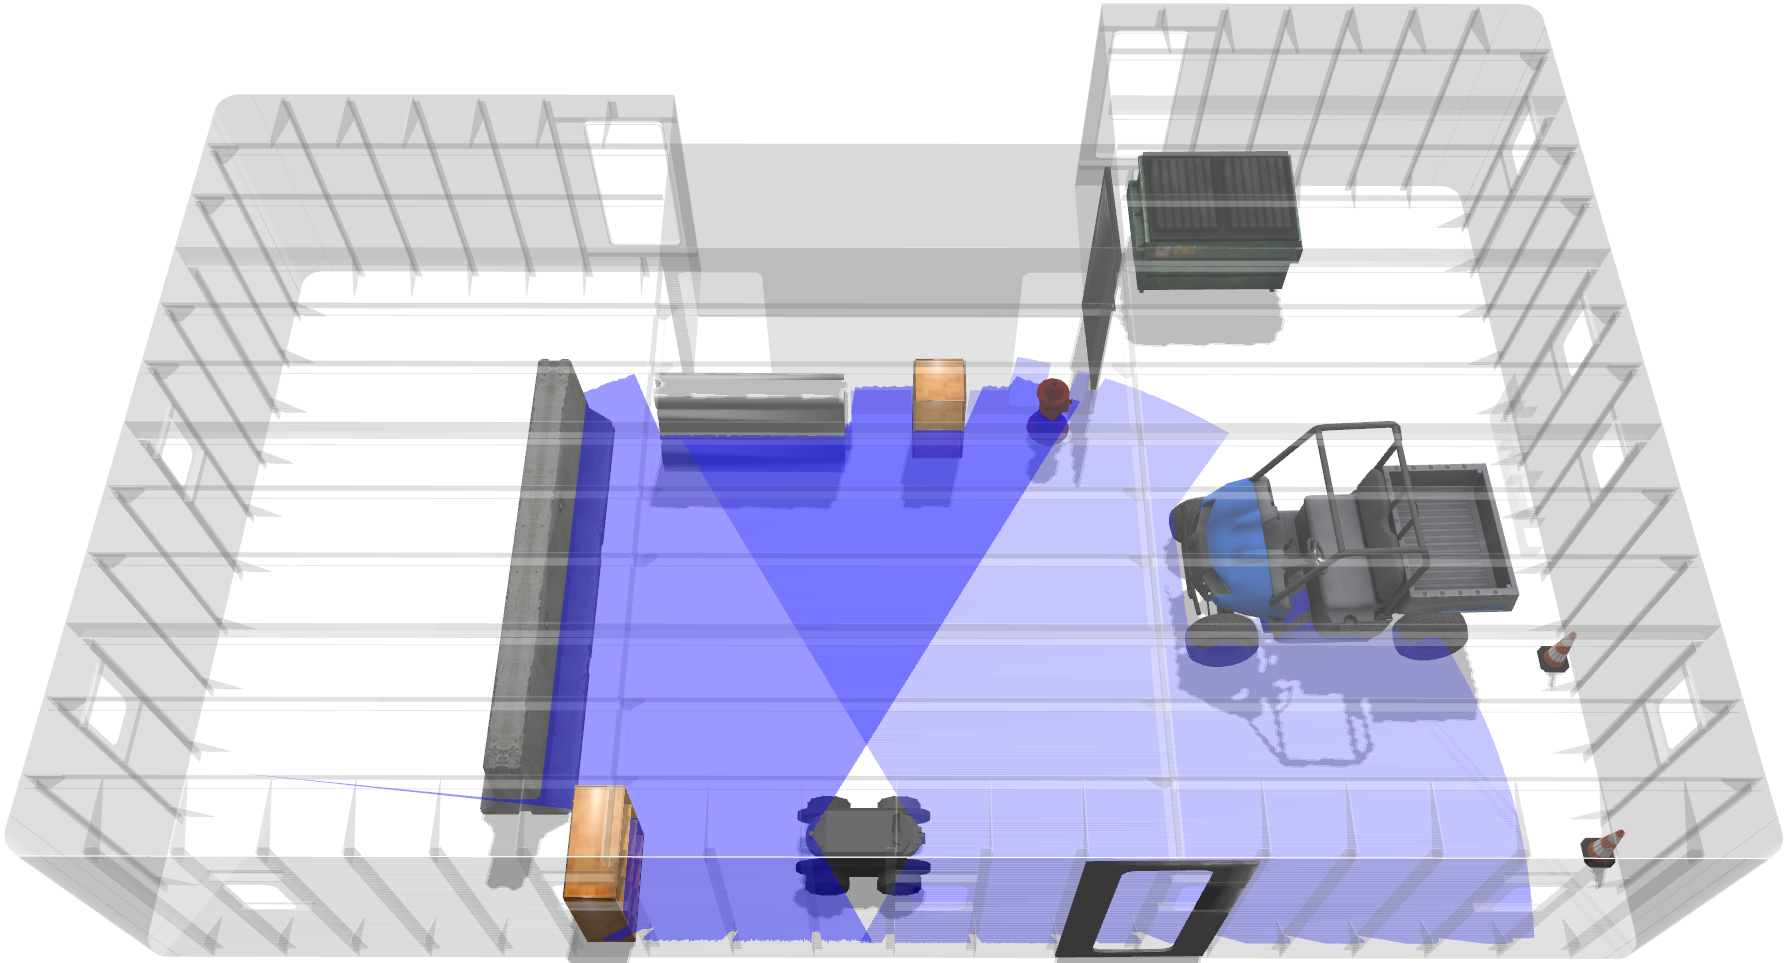
\includegraphics[width=\textwidth]{guardian-environment-cluttered-dynamic}
		\caption{\small Ambiente dinâmico}
		\label{fig:guardian-environment}
	\end{minipage}\hfill
	\begin{minipage}[b]{0.23\textwidth}
		\centering
		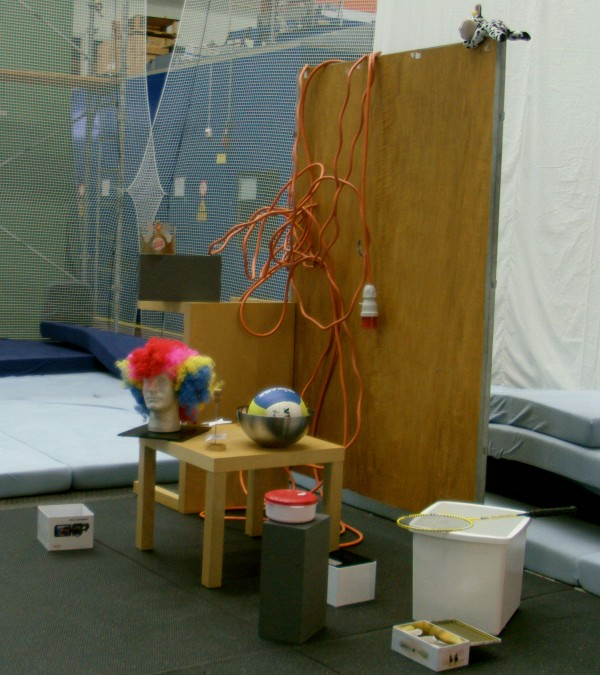
\includegraphics[width=0.6\textwidth]{kinect-flying-arena}
		\caption{\small Arêna de voo \cite{Pomerleau2011}}
		\label{fig:kinect-environment}
	\end{minipage}
\end{figure}



\section{Principais resultados}

O sistema de localização proposto é capaz de fazer a estimação da pose de plataformas robóticas móveis com menos de 1-2 centímetros de erro de translação e menos de um 1-3 graus de erro de rotação (em 3 e 6 DoF respetivamente) mesmo quando o robô / sensores se movimentam a velocidades elevadas em ambientes dinâmicos. Além disso, quando o rastreamento da pose é perdido ou nenhuma posição inicial é dada, o sistema é capaz de encontrar uma estimativa da pose global usando algoritmos de registo de características geométricas do ambiente. Esta abordagem permite alcançar rastreamento da pose de forma rápida e eficiente e consegue fazer a estimativa da pose inicial quando se revela necessário, proporcionando também o conjunto das poses iniciais aceites antes do refinamento do registo da nuvem do ambiente com a nuvem de referência, o que pode ser informação bastante valiosa para um supervisor de navegação quando o robô está numa região ambígua que pode ser registada em zonas semelhantes do mapa. O sistema permite também a reconfiguração dinâmica do número de varrimentos laser a agregar, de forma a atenuar os erros de medição dos sensores e adaptar a sua taxa de funcionamento de acordo com a velocidade estimada do robô.


\section{Conclusões}

A alta precisão alcançada pelo sistema de localização proposto, juntamente com a capacidade de atualização dinâmica do mapa e dado não necessitar de marcadores artificiais / modificações do ambiente, permitirá o rápido desenvolvimento de robôs móveis capazes de operar com segurança e precisão em ambientes dinâmicos.


\section{Trabalho futuro}

A implementação atual do sistema de localização pode ser melhorada com suporte para GPU a fim de alcançar taxas de atualização mais altas em 6 DoF e também com algoritmos de fechamento de laço, de forma a tornar-se um sistema de SLAM completo e permitir a criação de mapas precisos de ambientes de largas dimensões. Além disso, pode ser estendida para suportar localização baseada em imagem e percepção semântica do ambiente.


\bibliographystyle{unsrt-pt}
\bibliography{references}

\end{multicols}

\end{document}
